\documentclass[10pt]{article}
\usepackage{amsmath}
\usepackage{amsfonts}
\usepackage{latexsym}
\usepackage[pdftex]{graphicx}
\usepackage{fullpage}
\usepackage{subfigure}

\newcommand{\degree}{\ensuremath{^\circ}}

\title{\texttt{LogoBot}: A new platform for educational robotics}
\author{A product of NUBlabs}
\date{Last edited \today}

\begin{document}

\maketitle
\section{Overview}
NUBlabs is a local design collective excited about empowering communities through education and technology.  As part of that mission, we do custom engineering and design for schools and other socially aware organizations.

We've been working on an idea of our for a while.  We want to design and build a small, affordable, wireless robot that understands the programming language Logo (LogoBot!) and create online support materials that can be grown over time by teachers and their students.

NUBlabs is looking for a school interested enough in LogoBot and the accompanying support materials we'd like to create to sponsor the initial engineering and material costs.  Our hope is that by finding and satisfying school's needs in a flexible way, we can sustain ourselves by offering those solutions to the sponsor school at or below cost, and then offer the finished product as a kit and/or product to the wider educational community.

If you're interested in being involved in this project (or if there's anything else with which NUBlabs might be able to help you), please don't hesitate to get in touch with us!
  
\section{Logo}
Logo uses simple commands like \texttt{forward}, \texttt{right}, \texttt{left}, \texttt{pen up}, \texttt{pen down}, and so on.\footnote{\texttt{http://en.wikipedia.org/wiki/Logo\_programming\_language}} to control a virtual or physical avatar that can move and draw.  Historically, this avatar has been a ``turtle'' either on screen (see Figure \ref{turtleart}) or in real life (see Figure \ref{logobot-cad} for a CAD model of a preliminary design).  

Logo aims to make programming and logic physically intuitive by capitalizing on the way we already think about motion to introduce advanced programming, mathematical, and epistemological concepts.  The pedagogical versatility and value of the language was explored in Seymour Papert's \textit{Mindstorms}.\footnote{If you're interested in exploring Papert's ideas about constructionism more deeply, NUBlabs would be happy to donate or loan a copy of \textit{Mindstorms} to you.}

\begin{figure}
\centering
\subfigure[An example of the virtual LogoBot included on the XO laptop of the One Laptop Per Child program]{\label{turtleart}
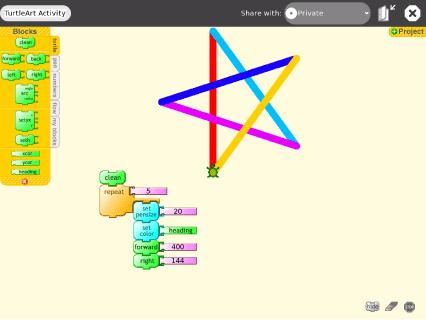
\includegraphics[height=2in]{turtleArt.jpg}}
\subfigure[A preliminary CAD drawing of our design for LogoBot]{\label{logobot-cad}
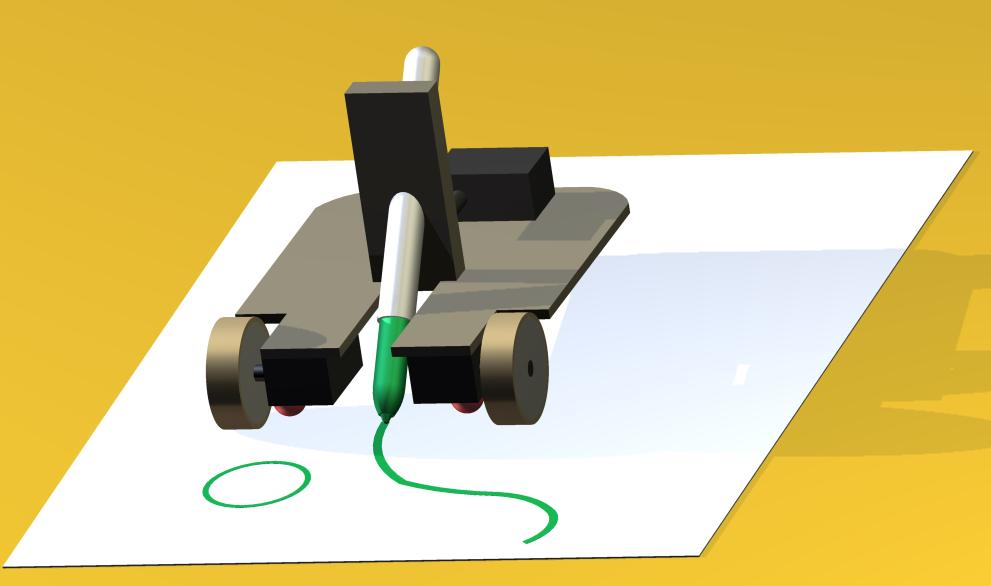
\includegraphics[height=2in]{logobot-cad-v0.jpg}}
\end{figure}

\section{LogoBot}
LogoBot's size and cost would make it a candidate for developing an educational platform from which to explore swarm computing and emergent phenomena in a physical environment.  Currently, swarm computing is prohibitively expensive and relatively unapproachable.  Environments like StarLogo\footnote{\texttt{http://education.mit.edu/starlogo/}} have made it possible (though not particularly easy) for students to play with complex, emergent systems.  LogoBot can bring physicality to the process.

Our world is increasingly one comprising complex systems whose principles of behavior are not always immediately obvious.  Although we've recognized the need to incorporate complex systems behavior into our curricula, there is much left to do.  Mitch Resnick, principal investigator of the MIT Media Lab's Lifelong Kindergarten group, recently wrote a book entitled \textit{Turtles, Termites, and Traffic Jams: Explorations in Massively Parallel Microworlds} that addresses the need and opportunity to explore this domain with children.\footnote{Once again, if you're interested in exploring this more deeply, NUBlabs would be happy to donate or loan a copy to you.}

LogoBot will be designed interface with the MIT Media Lab's Scratch programming environment\footnote{\texttt{http://scratch.mit.edu}}, which means there will be a tremendous community excited and ready to explore LogoBot.  Through the plugin we'll write, people familiar with Scratch will be able to write programs for LogoBot in Scratch and execute them seamlessly.  Depending on support and interest from the MIT Media Lab, it is even possible that the LogoBot programs could be shared and remixed as the current Scratch programs are, on the Scratch website.

LogoBot will offer a quick, versatile platform on which to explore robotics, computing, and a host of mathematical concepts.  Our aim is to make this as pedagogically valuable a product as possible. For instance, given that NUBlabs will be offering LogoBot both as a completed project and as an open source kit, constructing LogoBot from scratch would be a fantastic context for teaching basic electronics, culminating in a functional, powerful robot.
  
Beyond this, Logo was designed with the goal of teaching programming and logic in mind.  With an affordable, flexible, extensible tool like Logobot, teaching programming to students in an exciting, engaging environment that encourages iteration and debugging, rather than convergent, test-based thinking becomes an option.  Because of Logo's age and the active community surrounding the various Logo-based initiatives, there is a plethora of teaching materials and activities that can be reappropriated and remixed.

And LogoBot is not aimed just at children; there has been extensive work using Logo to teach higher level mathematics.  Abelson and di Sessa's \textit{Turtle Geometry} walks the reader from the basics of Logo all the way through differential geometry and general relativity.

In short, Logo and LogoBot, combined with the resources offered by the existing Scratch and Logo communities, presents an exciting opportunity for teachers and students to bring a versatile, well-supported tool to education.
\end{document}